\documentclass[12 pt]{article}
\usepackage[utf8]{inputenc}
\usepackage{matlab-prettifier}
\usepackage[portuguese]{babel}
\usepackage{indentfirst}
\usepackage{graphicx}
\usepackage{float}
\usepackage{subcaption}
\usepackage[font=small,labelfont=bf]{caption}
\definecolor{mygreen}{RGB}{28,172,0} % color values Red, Green, Blue
\definecolor{myyellow}{rgb}{1.0, 1.0, 0.8}
\usepackage{mathtools}
\usepackage{multirow}
\usepackage{comment}
\usepackage{xcolor}
\usepackage{colortbl}
\usepackage[normalem]{ulem}               % to striketrhourhg text
\usepackage{amsmath}
\usepackage{amsfonts}
\usepackage{hyperref}
\usepackage{tcolorbox}
\usepackage{longtable}
\usepackage{enumitem}
\newcommand\redout{\bgroup\markoverwith
{\textcolor{red}{\rule[0.5ex]{2pt}{0.8pt}}}\ULon}
\renewcommand{\lstlistingname}{Código}% Listing -> Algorithm
\renewcommand{\lstlistlistingname}{Lista de \lstlistingname s}% List of Listings -> List of Algorithms

\usepackage[top=3cm,left=2cm,bottom=2cm, right=2cm]{geometry}
\usepackage{tikz}
\usetikzlibrary{decorations.pathreplacing}
\usetikzlibrary{automata}
\usetikzlibrary{positioning}
\usetikzlibrary{arrows.meta, positioning}

\usepackage{adjustbox}


% Configuração para destacar a sintaxe do Python
\lstset{ 
    language=Python,                     % A linguagem do código
    backgroundcolor=\color{myyellow}, % A cor do fundo 
    basicstyle=\ttfamily\footnotesize,   % O estilo do texto básico
    keywordstyle=\color{blue},           % Cor das palavras-chave
    stringstyle=\color{red},             % Cor das strings
    commentstyle=\color{mygreen},          % Cor dos comentários
    numbers=left,                        % Números das linhas à esquerda
    numberstyle=\tiny\color{gray},       % Estilo dos números das linhas
    stepnumber=1,                        % Número de linhas entre os números das linhas
    frame=single,                        % Moldura ao redor do código
    breaklines=true,                     % Quebra automática das linhas longas
    captionpos=t,                        % Posição da legenda
    showstringspaces=false               % Não mostra espaços em branco nas strings
    extendedchars=true,
    literate={º}{{${ }^{\underline{o}}$}}1 {á}{{\'a}}1 {à}{{\`a}}1 {ã}{{\~a}}1 {é}{{\'e}}1 {É}{{\'E}}1 {ê}{{\^e}}1 {ë}{{\"e}}1 {í}{{\'i}}1 {ç}{{\c{c}}}1 {Ç}{{\c{C}}}1 {õ}{{\~o}}1 {ó}{{\'o}}1 {ô}{{\^o}}1 {ú}{{\'u}}1 {â}{{\^a}}1 {~}{{$\sim$}}1
}


\title{%
\textbf{\huge Universidade Federal do Rio de Janeiro} \par
\textbf{\LARGE Instituto Alberto Luiz Coimbra de Pós-Graduação e Pesquisa de Engenharia} \par


\includegraphics[width=8cm]{COPPE UFRJ.png} \par

\textbf{Programa de Engenharia de Sistemas e Computação} \par

COS868 - Probabilidade e Estatística para Aprendizado de Máquina \par

Profa. Dra. Rosa M. Leão (PESC/COPPE/UFRJ)\par

\vspace{1\baselineskip}
\textbf{\textit{Projeto do Curso}} \par
}

\author{Luiz Henrique Souza Caldas\\email: lhscaldas@cos.ufrj.br}

\date{\today}

\begin{document}
\maketitle

\tableofcontents

\section{Introdução}

\subsection{Objetivo}

O objetivo deste trabalho é realizar uma análise de um conjunto de dados reais fornecidos por um provedor de Internet de médio porte, avaliando as taxas de upload e download de dispositivos domésticos, especificamente Smart-TVs e Chromecasts, com base na teoria aprendida em classe, destacando a importância de uma análise crítica dos resultados obtidos.

\subsection{Análise Exploratória dos Dados}\label{sec:eda}

A análise exploratória foi realizada para compreender as características principais dos dados obtidos dos dispositivos Smart TV e Chromecast. Os resultados estão detalhados abaixo:

\begin{itemize}
    \item \textbf{Primeiras linhas dos dados:}
    \begin{itemize}
        \item \textbf{Smart TV:}
        \begin{verbatim}
            device_id            date_hour       bytes_up    bytes_down
        0   77209603  2021-11-22 15:23:00  132932.983607  2.818140e+06
        1   77209603  2021-11-22 15:24:00  115770.491803  2.264410e+06
        2   77209603  2021-11-22 15:25:00  114030.032787  2.309270e+06
        3   77209603  2021-11-22 15:26:00   97170.622951  2.006544e+06
        4   77209603  2021-11-22 15:27:00   39569.573770  8.061440e+05
        \end{verbatim}
        
        \item \textbf{Chromecast:}
        \begin{verbatim}
            device_id            date_hour     bytes_up    bytes_down
        0   66161985  2021-09-06 00:01:00  2987.016393  49185.704918
        1   66161985  2021-09-06 00:02:00   685.935484    328.258065
        2   66161985  2021-09-06 00:03:00  4493.901639  37914.064516
        3   66161985  2021-09-06 00:04:00   776.133333    229.200000
        4   66161985  2021-09-06 00:05:00  3081.311475  51656.800000
        \end{verbatim}
    \end{itemize}
    
    \item \textbf{Dimensões dos dados:}
    \begin{itemize}
        \item Smart TV: (4417903, 4)
        \item Chromecast: (1620529, 4)
    \end{itemize}

    \item \textbf{Dados faltantes:}
    \begin{itemize}
        \item Smart TV: Nenhum valor faltante em \texttt{device\_id}, \texttt{date\_hour}, \texttt{bytes\_up}, \texttt{bytes\_down}.
        \item Chromecast: Nenhum valor faltante em \texttt{device\_id}, \texttt{date\_hour}, \texttt{bytes\_up}, \texttt{bytes\_down}.
    \end{itemize}

    \item \textbf{Valores zero:}
    \begin{itemize}
        \item Smart TV: \texttt{bytes\_up} = 1.803.853, \texttt{bytes\_down} = 1.978.337.
        \item Chromecast: \texttt{bytes\_up} = 6.057, \texttt{bytes\_down} = 4.099.
    \end{itemize}

    \item \textbf{Valores negativos:}
    \begin{itemize}
        \item Smart TV: Nenhum valor negativo em \texttt{bytes\_up} ou \texttt{bytes\_down}.
        \item Chromecast: Nenhum valor negativo em \texttt{bytes\_up} ou \texttt{bytes\_down}.
    \end{itemize}
\end{itemize}


\subsection{Pré-processamento}

O pré-processamento foi realizado para preparar os dados dos dispositivos Smart TV e Chromecast para análises posteriores. As etapas realizadas são descritas a seguir:

\begin{itemize}
    \item \textbf{Carregamento dos dados:} Os dados foram lidos a partir dos arquivos \texttt{dataset\_smart-tv.csv} e \texttt{dataset\_chromecast.csv}.

    \item \textbf{Correção de valores zero:} Como as colunas \texttt{bytes\_up} e \texttt{bytes\_down} apresentavam valores zero, foi aplicado um \textit{shift} de +1 a todos os valores dessas colunas para evitar problemas no cálculo do logaritmo.

    \item \textbf{Reescalonamento dos dados:} Os valores das colunas \texttt{bytes\_up} e \texttt{bytes\_down} foram transformados para a escala logarítmica na base 10 (\texttt{log10}), devido à grande variação na ordem de grandeza desses valores.

    \item \textbf{Ordenação temporal:} Os dados foram ordenados pela coluna \texttt{date\_hour} para garantir a consistência temporal nas análises subsequentes.

    \item \textbf{Salvamento dos dados processados:} Os datasets resultantes podem ser salvos como arquivos CSV (\texttt{smart\_preprocessado.csv} e \texttt{chrome\_preprocessado.csv}) para uso posterior.
\end{itemize}

Essa etapa garante que os dados estejam limpos, reescalonados e organizados, facilitando análises estatísticas e a geração de gráficos. Além disso, a transformação logarítmica reduz a influência de valores extremos, melhorando a interpretação dos resultados. 

\section{Estatísticas Gerais}

Nesta seção, são apresentadas as estatísticas gerais dos dados coletados para os dispositivos \textit{Smart-TV} e \textit{Chromecast}. As análises incluem cálculos de medidas descritivas, como média, variância e desvio padrão, além de representações gráficas através de histogramas, boxplots e funções de distribuição empírica (ECDF). 

\subsection{Medidas Descritivas}

As medidas descritivas para as taxas de \textit{upload} e \textit{download} (em escala logarítmica base 10) estão resumidas na Tabela~\ref{tab:estatisticas}. 

\begin{table}[H]
\centering
\caption{Medidas descritivas das taxas de \textit{upload} e \textit{download}.}
\label{tab:estatisticas}
\begin{tabular}{|c|c|c|c|c|}
\hline
\textbf{Dispositivo} & \textbf{Tipo de Tráfego} & \textbf{Média} & \textbf{Variância} & \textbf{Desvio Padrão} \\ \hline
\textit{Smart-TV} & \textit{Upload} & 2.16 & 4.11 & 2.03 \\ \hline
\textit{Smart-TV} & \textit{Download} & 2.35 & 6.72 & 2.59 \\ \hline
\textit{Chromecast} & \textit{Upload} & 3.35 & 0.46 & 0.68 \\ \hline
\textit{Chromecast} & \textit{Download} & 3.80 & 1.66 & 1.29 \\ \hline
\end{tabular}
\end{table}

\subsection{Visualizações Gráficas}

Para compreender melhor a distribuição dos dados, são utilizadas as seguintes representações gráficas:

\begin{itemize}
    \item \textbf{Histogramas:} As distribuições das taxas de \textit{upload} e \textit{download} para cada dispositivo estão representadas nos histogramas da Figura~\ref{fig:histogramas}.
    \item \textbf{Boxplots:} A Figura~\ref{fig:boxplots} mostra os boxplots comparando as taxas de \textit{upload} e \textit{download} entre \textit{Smart-TV} e \textit{Chromecast}.
    \item \textbf{ECDF:} As funções de distribuição empírica, exibidas na Figura~\ref{fig:ecdf}, demonstram a probabilidade acumulada para cada valor das taxas.
\end{itemize}

Para a construção dos histogramas, o número de bins foi calculado utilizando o método de Sturges:

\begin{equation}\label{eq:sturges}
k = 1 + \log_2(n),
\end{equation}

onde \(n\) é o número total de amostras. Este método busca otimizar a visualização dos dados ao balancear granularidade e clareza.

O número de bins calculado para cada dispositivo é o seguinte:
\begin{itemize}
    \item \textbf{\textit{Smart-TV}:} \(k = 24\) bins.
    \item \textbf{\textit{Chromecast}:} \(k = 22\) bins.
\end{itemize}

\begin{figure}[H]
    \centering
    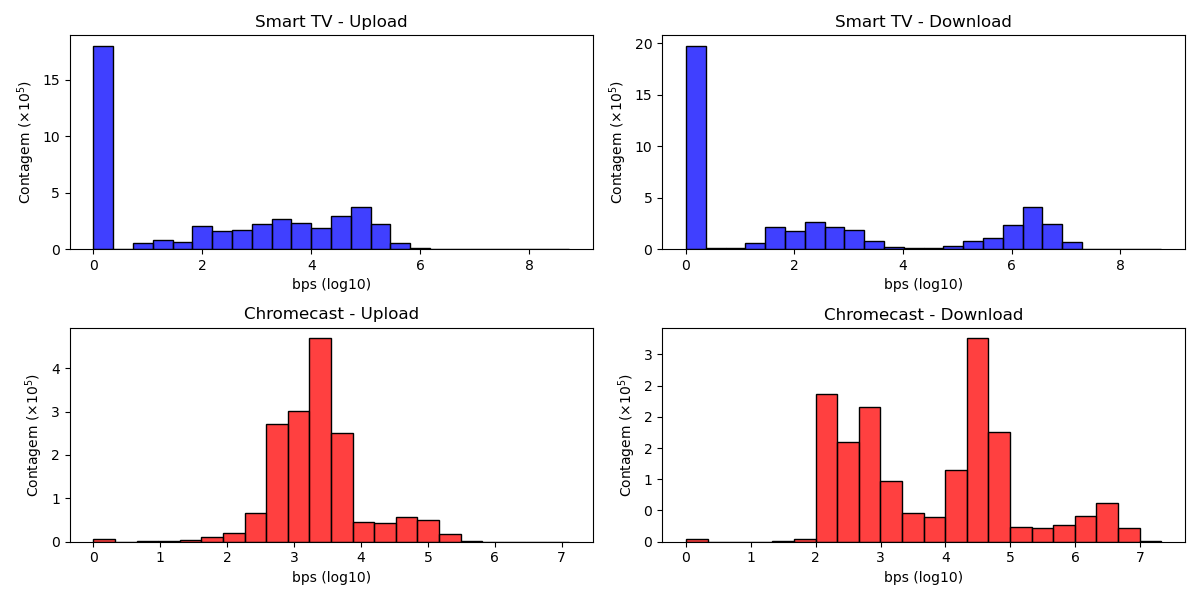
\includegraphics[width=0.8\textwidth]{../estatísticas gerais/histogramas.png}
    \caption{Histogramas das taxas de \textit{upload} e \textit{download} para \textit{Smart-TV} e \textit{Chromecast}.}
    \label{fig:histogramas}
\end{figure}

\begin{figure}[H]
    \centering
    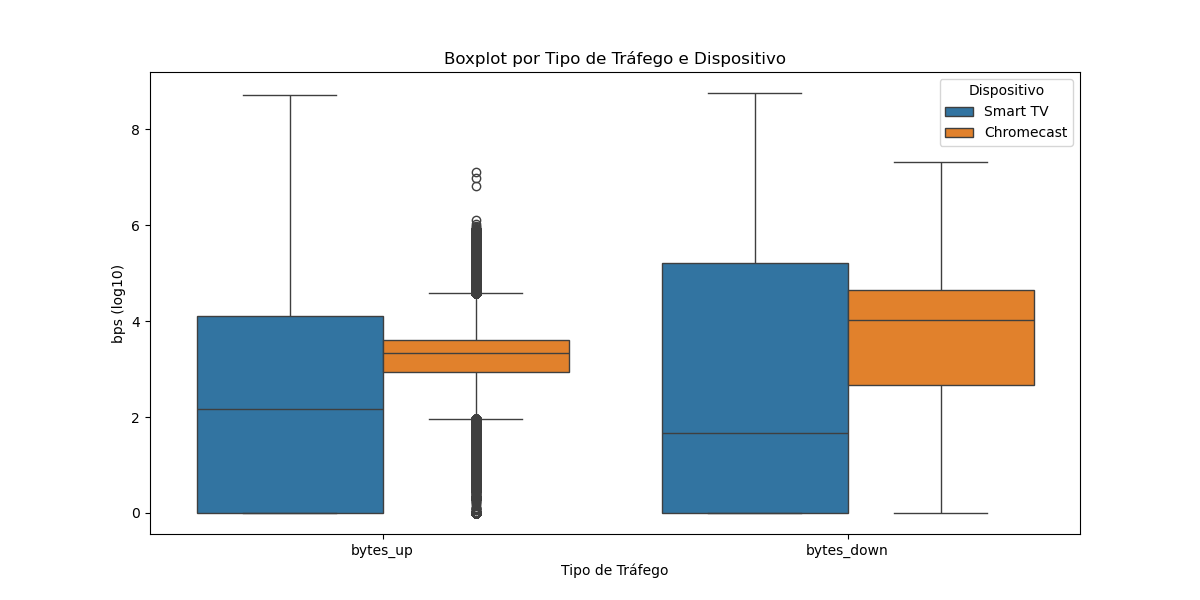
\includegraphics[width=0.8\textwidth]{../estatísticas gerais/boxplot.png}
    \caption{Boxplots das taxas de \textit{upload} e \textit{download} para \textit{Smart-TV} e \textit{Chromecast}.}
    \label{fig:boxplots}
\end{figure}

\begin{figure}[H]
    \centering
    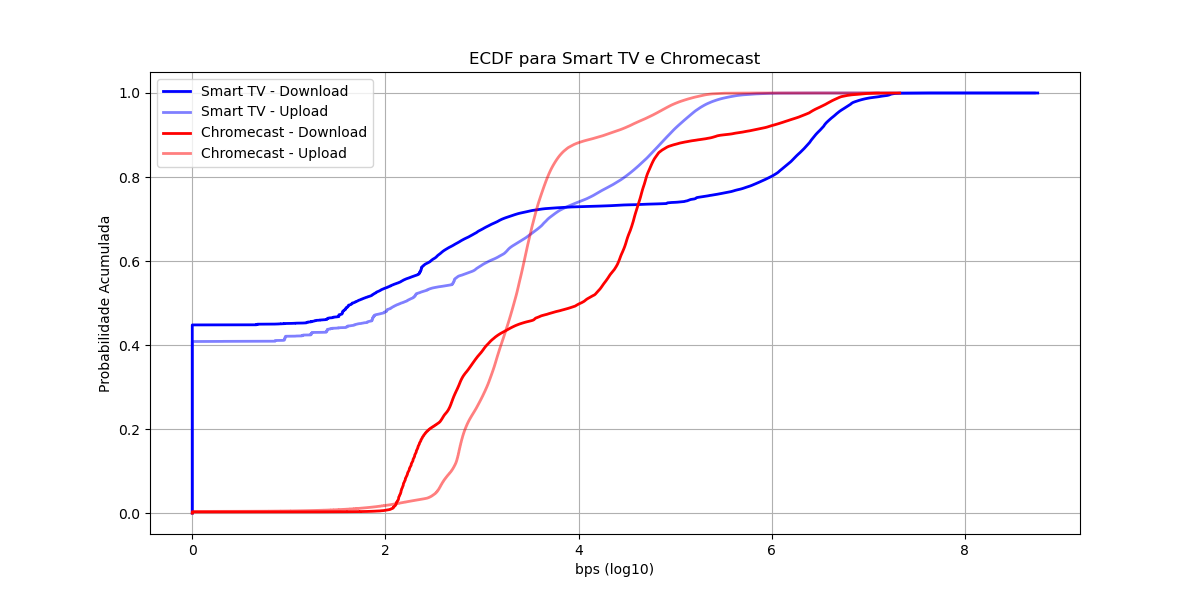
\includegraphics[width=0.8\textwidth]{../estatísticas gerais/ecdf.png}
    \caption{Funções de Distribuição Empírica (ECDF) das taxas de \textit{upload} e \textit{download}.}
    \label{fig:ecdf}
\end{figure}

As visualizações gráficas fornecem informações importantes para o provedor de serviços ao identificar padrões de tráfego específicos de cada dispositivo. Por exemplo, histogramas permitem entender a distribuição predominante de dados, enquanto os boxplots destacam possíveis valores atípicos que podem impactar negativamente a rede. Essas análises auxiliam na definição de prioridades no gerenciamento do tráfego de rede, garantindo uma melhor alocação de recursos para dispositivos com padrões mais variáveis.

\subsection{Análise dos Resultados}

Os resultados destacam diferenças importantes nas características das taxas de \textit{upload} e \textit{download} entre os dispositivos \textit{Smart-TV} e \textit{Chromecast}, com implicações práticas significativas para o provedor de serviços de Internet.

\textbf{\textit{Smart-TV}:} As taxas de \textit{upload} e \textit{download} da \textit{Smart-TV} apresentam médias similares e variâncias relativamente altas, refletindo maior dispersão dos dados. A alta concentração de valores baixos, especialmente iguais a zero, é evidenciada pela primeira barra dominante nos histogramas (Figura~\ref{fig:histogramas}) e pela ECDF inicial, que ultrapassa 0.4 devido aos valores nulos. O boxplot (Figura~\ref{fig:boxplots}) confirma a ausência de outliers, indicando que o tráfego da \textit{Smart-TV} é caracterizado por períodos de inatividade alternados com picos de alta demanda. 

\textbf{\textit{Chromecast}:} O \textit{Chromecast} apresenta padrões diferentes, com taxas de \textit{upload} e \textit{download} mais consistentes e desvios padrão menores. Embora a taxa de \textit{download} não tenha outliers, a taxa de \textit{upload} exibe diversos picos e vales, refletidos nos boxplots. A ECDF mostra um crescimento rápido após \(10^2\) bps, indicando concentração em valores intermediários e reforçando o comportamento mais estável do dispositivo.

\textbf{Comparação Geral:} Enquanto a \textit{Smart-TV} alterna entre inatividade e fluxos intensos, o \textit{Chromecast} mantém tráfego mais constante, mas com picos significativos no \textit{upload}. Essas diferenças sugerem abordagens específicas para otimização da rede: adaptar a alocação de recursos às demandas variáveis da \textit{Smart-TV} e conter os picos do \textit{Chromecast}, priorizando a estabilidade.

\textbf{Implicações Práticas:} Os padrões observados podem ajudar o provedor de serviços a otimizar sua infraestrutura. Para a \textit{Smart-TV}, estratégias adaptativas para lidar com períodos de alta demanda podem reduzir a sobrecarga durante picos. Já para o \textit{Chromecast}, sistemas de contenção que lidem com os picos de \textit{upload} podem evitar saturação da rede. A implementação dessas políticas pode melhorar a eficiência operacional e a qualidade da experiência (QoE) do usuário final.


\section{Códigos}

Os códigos utilizados em todas as etapas deste projeto estão disponíveis no repositório do GitHub: \url{https://github.com/lhscaldas/Projeto_Probabilidade_e_Estatistica}

\bibliographystyle{abntex2-num} % Escolha o estilo de citação desejado
\nocite{Kobayashi_2011}
\nocite{Pishro_2014}
\bibliography{bibliografia} % Nome do arquivo .bib (sem a extensão)

\end{document}